\documentclass[letter,11pt]{article}

\usepackage[spanish,es-nodecimaldot]{babel}
\usepackage[utf8]{inputenc}

\renewcommand{\familydefault}{\sfdefault}
\usepackage[T1]{fontenc}
\usepackage{textcomp}

\usepackage{framed}
\usepackage[svgnames]{xcolor}
\colorlet{shadecolor}{Gainsboro!50}

\usepackage{enumitem}
\usepackage{graphicx}
\usepackage{pstricks}

\usepackage{anysize}
\marginsize{3cm}{2cm}{2cm}{3cm}

\usepackage{float}
\usepackage{siunitx}
\usepackage{amsmath}
\usepackage{array}
\usepackage{alltt}

\usepackage{fancyhdr}
\usepackage{lastpage}
\pagestyle{fancy}
\fancyhf{}
\fancyhead[LE,RO]{Termodinámica}
\fancyfoot[CO,CE]{\thepage\ de \pageref{LastPage}}

\special{papersize=215.9mm,279.4mm}

\usepackage[
    pdfauthor={Carlos Eduardo Caballero Burgoa},%
    pdftitle={Termodinámica},%
    pdfsubject={Practica 04},%
    colorlinks,%
    citecolor=black,%
    filecolor=black,%
    linkcolor=black,%
    urlcolor=black,
    breaklinks]{hyperref}
\usepackage{breakurl}

\renewcommand{\arraystretch}{1.2}

\begin{document}

\begin{center}
    {\Large \bf{Practica \#04}}
\end{center}

\begin{enumerate}
\item Un cilindro con su embolo inicialmente contiene $1[m^3]$ de agua a
$75^\circ C$. El $50\%$ del volumen esta en estado liquido saturado y el resto
como vapor saturado. El embolo pesa $400[kg]$ y su diámetro es de $20[cm]$, la
presión atmosférica es de $101[kPa]$. En el estado inicial hallar el titulo de
la mezcla, y la masa total del agua. Se entrega calor al agua hasta que su
temperatura sea de $200^\circ C$. Hallar el calor entregado al agua.

\begin{figure}[H]
\centering
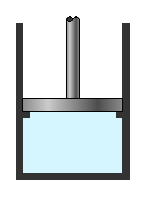
\includegraphics[scale=1.2]{resources/f01.eps}
\end{figure}

\textbf{\underline{Solución}:} \\

\underline{Datos provistos:}
\begin{equation*}
    \text{Agua}
\end{equation*}
\begin{equation*}
    V = 1[m^3]
\end{equation*}
\begin{equation*}
    m_E=400[kg]
\end{equation*}
\begin{equation*}
    d_E=0.2[m]
\end{equation*}
\begin{equation*}
    T_1=75^\circ C
\end{equation*}
\begin{equation*}
    V_l=0.5V
\end{equation*}
\begin{equation*}
    V_v=0.5V
\end{equation*}
\begin{equation*}
    P_{atm}=101[kPa]
\end{equation*}
\begin{equation*}
    T_3=200^\circ C
\end{equation*}

\underline{Estado 1}: \\
De Tablas Termodinámicas se obtienen los valores para una temperatura de
$75^\circ C$:

\begin{equation*}
    T(75^\circ C) = \begin{cases}
        P = 38.58[kPa] \\
        \nu_l = 0.001026[m^3/kg] & u_l = 313.87[kJ/kg] \\
        \nu_v = 4.13123[m^3/kg]  & u_v = 2475.91[kJ/kg]
    \end{cases}
\end{equation*}

Se halla la masa liquida, de vapor y total del agua a partir de sus volúmenes
específicos:

\begin{equation*}
    m_l = \frac{V_l}{\nu_l} = \frac{0.5[m^3]}{0.001026[m^3/kg]} = 487.33[kg]
\end{equation*}
\begin{equation*}
    m_v = \frac{V_v}{\nu_v} = \frac{0.5[m^3]}{4.13123[m^3/kg]} = 0.12[kg]
\end{equation*}
\begin{equation*}
    m = m_l + m_v = 487.3294[kg] + 0.12103[kg] = 487.45[kg]
\end{equation*}

Se halla el titulo a partir de su definición:

\begin{equation*}
    X = \frac{m_v}{m} = \frac{0.121[kg]}{487.45[kg]} = 0.0002
\end{equation*}

Se calcula el volumen especifico a partir del titulo:

\begin{equation*}
    \begin{split}
        \nu &= \nu_l + X(\nu_v - \nu_l) \\
            &= 0.001026[m^3/kg] + 0.0002(4.13123[m^3/kg] - 0.001026[m^3/kg]) \\
            &= 0.00205[m^3/kg]
    \end{split}
\end{equation*}

Se calcula la energía interna a partir del titulo:

\begin{equation*}
    \begin{split}
        u &= u_l + X(u_v - u_l) \\
          &= 313.87[kJ/kg] + 0.0002(2475.91[kJ/kg] - 313.87[kJ/kg]) \\
          &= 314.41[kJ/kg]
    \end{split}
\end{equation*}

\begin{figure}[H]
\centering
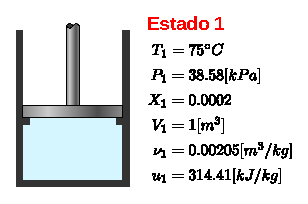
\includegraphics[scale=1.2]{resources/f01-1.eps}
\end{figure}

\underline{Estado 2}: \\
Se halla la presión que ejerce el embolo:

\begin{equation*}
    \begin{split}
        P &= P_{atm} + P_E  \\
          &= P_{atm} + \frac{F_E}{A_E} \\
          &= P_{atm} + \frac{m_E\,g}{\pi r_E^2} \\
          &= 101[kPa] + \frac{400[kg]\,9.8[m/s^2]}{\pi\,(0.1)^2[m^2]}
          \frac{1[kPa]}{1000[Pa]} \\
          &= 225.78[kPa]
    \end{split}
\end{equation*}

De Tablas Termodinámicas se obtienen los valores para una presión aproximada a
$225.78[kPa]$:

\begin{equation*}
    P(225[kPa]) = \begin{cases}
        T = 124^\circ C \\
        \nu_l = 0.001064[m^3/kg] & u_l = 520.45[kJ/kg] \\
        \nu_v = 0.79325[m^3/kg]  & u_v = 2533.56[kJ/kg]
    \end{cases}
\end{equation*}

Se halla el titulo a partir de su definición:

\begin{equation*}
    X = \frac{\nu-\nu_l}{\nu_v-\nu_l}
      = \frac{0.00205[m^3/kg] - 0.001064[m^3/kg]}
      {0.79325[m^3/kg] - 0.001064[m^3/kg]}
      = 0.0012
\end{equation*}

\begin{figure}[H]
\centering
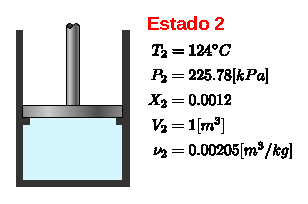
\includegraphics[scale=1.2]{resources/f01-2.eps}
\end{figure}

\underline{Estado 3}: \\
De Tablas Termodinámicas se obtienen los valores para una presión aproximada de
$225.78[kPa]$ y una temperatura de $200^\circ C$:

\begin{equation*}
    P(200[kPa])\,|\,T(200^\circ C) = \begin{cases}
        \nu = 1.08034[m^3/kg] \\
        u = 2654.39[kJ/kg]
    \end{cases}
\end{equation*}

Se halla el volumen a partir de la definición de volumen especifico:

\begin{equation*}
    V = \nu\,m = (1.08034[m^3/kg])(487.45[kg]) = 526.61[m^3]
\end{equation*}

\begin{figure}[H]
\centering
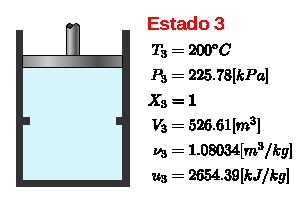
\includegraphics[scale=1.2]{resources/f01-3.eps}
\end{figure}

\underline{Trabajo}: \\
\begin{equation*}
    \begin{split}
    W_{1\rightarrow 3} &= W_{1\rightarrow 2} + W_{2\rightarrow 3} \\
                       &= \int_1^2 P_{1\rightarrow 2}\,dv
                          + \int_2^3 P_{2\rightarrow 3}\,dv \\
                       &= 0 + P_2 \int_2^3 dv \\
                       &= P_2\,(V\Biggr|_2^3) \\
                       &= P_2(V_3-V_2) \\
                       &= 225.78[kPa](526.61[m^3]-1[m^3]) \\
                       &= 118671.41[kJ]
    \end{split}
\end{equation*}

\underline{Calor}: \\
A partir de la primera ley de la termodinámica, se halla el calor entregado:

\begin{equation*}
    \Delta U_{1\rightarrow 3} = Q_{1\rightarrow 3} - W_{1\rightarrow 3}
\end{equation*}
\begin{equation*}
    \begin{split}
        Q_{1\rightarrow 3} &= \Delta U_{1\rightarrow 3} + W_{1\rightarrow 3} \\
                           &= m(u_3 - u_1) + W_{1\rightarrow 3} \\
                           &= 487.45[kg](2654.39[kJ/kg]
                              -314.41[kJ/kg])+118671.41[kJ] \\
                           &= 1259559.06[kJ]
    \end{split}
\end{equation*}

\begin{figure}[H]
\centering
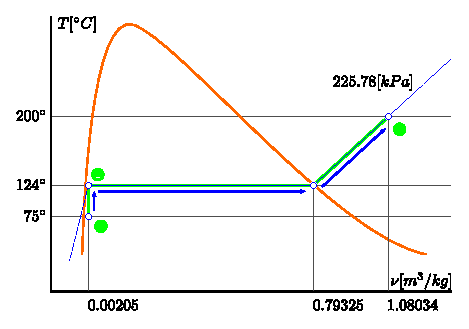
\includegraphics[scale=1.5]{resources/f01-d.eps}
\end{figure}

\begin{equation*}
\boxed{
    \begin{array}{l}
        Q = 1259559.06[kJ]
    \end{array}
}
\end{equation*}
\newpage

\item Se tiene $0.5[m^3]$ de amoniaco dentro un cilindro con su embolo a
$0.29[MPa]$ y $20^\circ C$, se colocan unos pesos sobre el embolo según la
figura hasta que el embolo llegue a los topes donde la presión llega a
$0.85[MPa]$ y $0.13[m^3]$. Durante este proceso la temperatura se mantiene
constante por que pierde calor al medio ambiente. Posteriormente el sistema
continua enfriándose hasta que la presión sea igual a la presión inicial.
Calcular 3 propiedades en cada estado.

\begin{figure}[H]
\centering
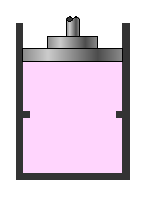
\includegraphics[scale=1.2]{resources/f02.eps}
\end{figure}

\textbf{\underline{Solución}:} \\

\underline{Datos provistos:}
\begin{equation*}
    \text{Amoniaco}
\end{equation*}
\begin{equation*}
    V_1 = 0.5[m^3]
\end{equation*}
\begin{equation*}
    P_1 = 290[kPa]
\end{equation*}
\begin{equation*}
    T_1 = 20^\circ C
\end{equation*}
\begin{equation*}
    V_2 = 0.13[m^3]
\end{equation*}
\begin{equation*}
    P_2=850[kPa]
\end{equation*}
\begin{equation*}
    T_2=20^\circ C
\end{equation*}
\begin{equation*}
    P_3=290[kPa]
\end{equation*}

\underline{Estado 1}: \\
De Tablas Termodinámicas se obtienen los valores para una presión aproximada a
$290[kPa]$:

\begin{equation*}
    P(290.9[kPa]) = \begin{cases}
        T = -10^\circ C
    \end{cases}
\end{equation*}

Por tanto, la sustancia se encuentra en la zona de vapor sobrecalentado.

De Tablas Termodinámicas se obtienen los valores para una presión aproximada de
$290[kPa]$ y una temperatura de $20^\circ C$:

\begin{equation*}
    P(300[kPa])\,|\,T(20^\circ C) = \begin{cases}
        \nu = 0.46077[m^3/kg] \\
        u = 1364.4[kJ/kg]
    \end{cases}
\end{equation*}

Se halla la masa total a partir de su volumen especifico:

\begin{equation*}
    m = \frac{V_l}{\nu_v} = \frac{0.5[m^3]}{0.46077[m^3/kg]}
      = 1.0851[kg]
\end{equation*}

\begin{figure}[H]
\centering
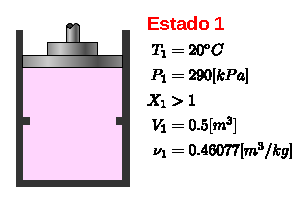
\includegraphics[scale=1.2]{resources/f02-1.eps}
\end{figure}

\underline{Estado 2}: \\
Se halla el volumen especifico a partir de su definición:

\begin{equation*}
    \nu = \frac{V}{m} = \frac{0.13[m^3]}{1.0851[kg]} = 0.1198[m^3/kg]
\end{equation*}

De Tablas Termodinámicas se obtienen los valores para una presión aproximada a
$850[kPa]$:

\begin{equation*}
    P(857.5[kPa]) = \begin{cases}
        T = 20^\circ C \\
        \nu_l = 0.001638[m^3/kg] & u_l = 272.89[kJ/kg] \\
        \nu_v = 0.14922[m^3/kg]  & u_v = 1332.2[kJ/kg]
    \end{cases}
\end{equation*}

Se halla el titulo a partir de su definición:

\begin{equation*}
    X = \frac{\nu-\nu_l}{\nu_v-\nu_l}
      = \frac{0.1198[m^3/kg] - 0.001638[m^3/kg]}
      {0.14922[m^3/kg] - 0.001638[m^3/kg]}
      = 0.8007
\end{equation*}

\begin{figure}[H]
\centering
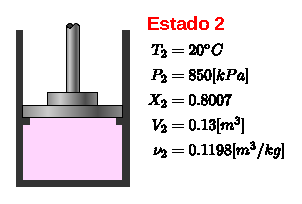
\includegraphics[scale=1.2]{resources/f02-2.eps}
\end{figure}

\underline{Estado 3}: \\
El volumen se mantiene constante.

\begin{equation*}
    V = 0.13[m^3]
\end{equation*}
\begin{equation*}
    \nu = 0.1198[m^3/kg]
\end{equation*}

De Tablas Termodinámicas se obtienen los valores para una presión aproximada a
$290[kPa]$:

\begin{equation*}
    P(290.9[kPa]) = \begin{cases}
        T = -10^\circ C \\
        \nu_l = 0.001534[m^3/kg] & u_l = 133.96[kJ/kg] \\
        \nu_v = 0.41808[m^3/kg]  & u_v = 1309.2[kJ/kg]
    \end{cases}
\end{equation*}

Se halla el titulo a partir de su definición:

\begin{equation*}
    X = \frac{\nu-\nu_l}{\nu_v-\nu_l}
      = \frac{0.1198[m^3/kg] - 0.001534[m^3/kg]}
      {0.41808[m^3/kg] - 0.001534[m^3/kg]}
      = 0.2839
\end{equation*}

\begin{figure}[H]
\centering
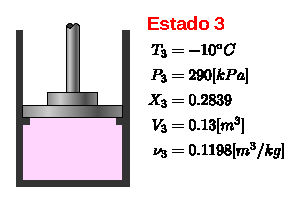
\includegraphics[scale=1.2]{resources/f02-3.eps}
\end{figure}

\begin{figure}[H]
\centering
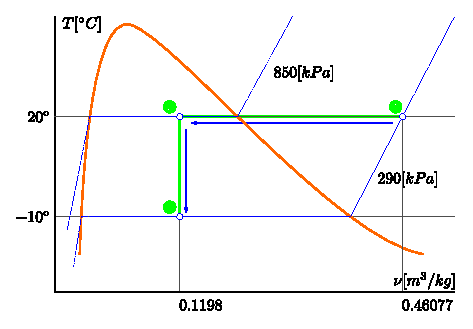
\includegraphics[scale=1.5]{resources/f02-d.eps}
\end{figure}
\newpage

\item Según la figura, se tiene agua como liquido saturado a $400[kPa]$ con un
volumen de $4.336[lt]$. Se entrega calor al agua hasta que su presión sea de
$1400[kPa]$. Posteriormente se enfría hasta que este como vapor saturado
permaneciendo el embolo en el mismo lugar. El volumen en los topes superiores es
de $1.2778[m^3]$. Hallar el calor intercambiado.

\begin{figure}[H]
\centering
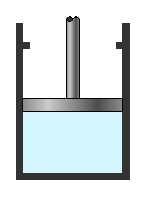
\includegraphics[scale=1.2]{resources/f03.eps}
\end{figure}

\textbf{\underline{Solución}:} \\

\underline{Datos provistos:}
\begin{equation*}
    \text{Agua}
\end{equation*}
\begin{equation*}
    P_1 = 400[kPa]
\end{equation*}
\begin{equation*}
    V_1 = 4.336[lt]\,\frac{0.001[m^3]}{1[lt]}=0.0043360[m^3]
\end{equation*}
\begin{equation*}
    X_1 = 0
\end{equation*}
\begin{equation*}
    P_3 = 1400[kPa]
\end{equation*}
\begin{equation*}
    X_4 = 1
\end{equation*}
\begin{equation*}
    V_4 = V_3
\end{equation*}
\begin{equation*}
    V_{max} = 1.2778[m^3]
\end{equation*}

\underline{Estado 1}: \\
De Tablas Termodinámicas se obtienen los valores para una presión de $400[kPa]$:

\begin{equation*}
    P(400[kPa]) = \begin{cases}
        T = 143.63^\circ C \\
        \nu_l = 0.001084[m^3/kg] & u_l = 604.29[kJ/kg] \\
        \nu_v = 0.46246[m^3/kg]  & u_v = 2553.55[kJ/kg]
    \end{cases}
\end{equation*}

Se halla la masa a partir de su volumen especifico:

\begin{equation*}
    m = \frac{V_l}{\nu_v} = \frac{0.0043360[m^3]}{0.001084[m^3/kg]}
      = 4.00[kg]
\end{equation*}

\begin{figure}[H]
\centering
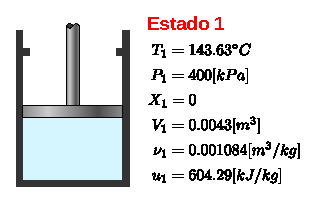
\includegraphics[scale=1.2]{resources/f03-1.eps}
\end{figure}

\underline{Estado 2}: \\
Se calcula el volumen especifico y el titulo cuando el embolo alcanza a los
topes:

\begin{equation*}
    \nu = \frac{V}{m} = \frac{1.2778[m^3]}{4[kg]} = 0.3194[m^3/kg]
\end{equation*}
\begin{equation*}
    X = \frac{\nu-\nu_l}{\nu_v-\nu_l}
      = \frac{0.3194[m^3/kg] - 0.001084[m^3/kg]}
      {0.46246[m^3/kg] - 0.001084[m^3/kg]}
      = 0.69
\end{equation*}

\begin{figure}[H]
\centering
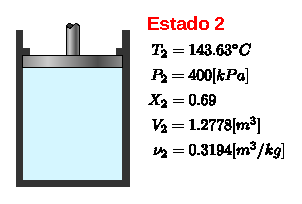
\includegraphics[scale=1.2]{resources/f03-2.eps}
\end{figure}

\underline{Estado 3}: \\
El volumen se mantiene constante.

\begin{equation*}
    V = 1.2778[m^3]
\end{equation*}
\begin{equation*}
    \nu = 0.3194[m^3/kg]
\end{equation*}

De Tablas Termodinámicas se obtienen los valores para una presión de
$1400[kPa]$:

\begin{equation*}
    P(1400[kPa]) = \begin{cases}
        T = 195.07^\circ C \\
        \nu_l = 0.001149[m^3/kg] & u_l = 828.68[kJ/kg] \\
        \nu_v = 0.14084[m^3/kg]  & u_v = 2592.83[kJ/kg]
    \end{cases}
\end{equation*}

Por tanto, la sustancia se encuentra en la zona de vapor sobrecalentado.

De Tablas Termodinámicas se obtienen los valores para una presión aproximada de
$1400[kPa]$ y un volumen especifico de $0.3194[m^3/kg]$:

\begin{equation*}
    P(1400[kPa])\,|\,\nu(0.31947[m^3/kg]) = \begin{cases}
        T = 700^\circ C \\
        u = 3473.61[kJ/kg]
    \end{cases}
\end{equation*}

\begin{figure}[H]
\centering
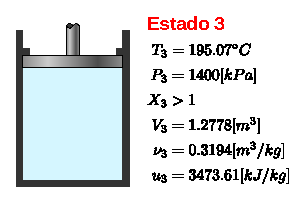
\includegraphics[scale=1.2]{resources/f03-3.eps}
\end{figure}

\underline{Estado 4}: \\
El volumen se mantiene constante.

\begin{equation*}
    \nu = 0.3194[m^3/kg]
\end{equation*}

De Tablas Termodinámicas se obtienen los valores para un volumen especifico de
$0.3194[m^3/kg]$ y un titulo de $1$:

\begin{equation*}
    \nu(0.31567[m^3/kg])\,|\,X(1) = \begin{cases}
        P = 600[kPa] \\
        T = 158.85^\circ C \\
        u = 2567.40[kJ/kg]
    \end{cases}
\end{equation*}

\begin{figure}[H]
\centering
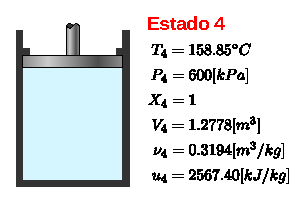
\includegraphics[scale=1.2]{resources/f03-4.eps}
\end{figure}

\underline{Trabajo}: \\
\begin{equation*}
    \begin{split}
    W_{1\rightarrow 4} &= W_{1\rightarrow 2} + W_{2\rightarrow 3}
                          + W_{3\rightarrow 4} \\
                       &= \int_1^2 P_{1\rightarrow 2}\,dv
                          + \int_2^3 P_{2\rightarrow 3}\,dv
                          + \int_3^4 P_{3\rightarrow 4}\,dv \\
                       &= P_1 \int_1^2 dv + 0 + 0 \\
                       &= P_1\,(V\Biggr|_1^2) \\
                       &= P_1(V_2-V_1) \\
                       &= 400[kPa](1.2778[m^3]-0.0043360[m^3]) \\
                       &= 509.39[kJ]
    \end{split}
\end{equation*}

\underline{Calor}: \\
A partir de la primera ley de la termodinámica, se halla el calor intercambiado:

\begin{equation*}
    \Delta U_{1\rightarrow 4} = Q_{1\rightarrow 4} - W_{1\rightarrow 4}
\end{equation*}
\begin{equation*}
    \begin{split}
        Q_{1\rightarrow 4} &= \Delta U_{1\rightarrow 4} + W_{1\rightarrow 4} \\
                           &= m(u_4 - u_1) + W_{1\rightarrow 4} \\
                           &= 4[kg](2567.40[kJ/kg]
                              -640.29[kJ/kg])+509.39[kJ] \\
                           &= 8361.8[kJ]
    \end{split}
\end{equation*}

\begin{figure}[H]
\centering
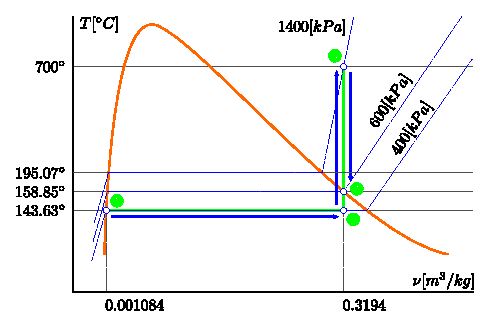
\includegraphics[scale=1.5]{resources/f03-d.eps}
\end{figure}

\begin{equation*}
\boxed{
    \begin{array}{l}
        Q = 8361.8[kJ]
    \end{array}
}
\end{equation*}
\newpage

\item Según la figura, el tanque $A$ tiene un volumen de $0.3[m^3]$ y contiene
freón 12 (R-12) como vapor saturado a $820[kPa]$. Cuando se abren las válvulas
el freón entra al cilindro $B$ en el cual se tiene un embolo que requiere una
presión de $200[kPa]$ para ser elevado. También entra freón al cilindro $C$ que
inicialmente también esta vacío cuyo embolo requiere una presión de $400[kPa]$
para ser elevado. El proceso termina cuando la presión se equilibra en los 3
recipientes. Durante el proceso en $B$ el embolo con área de $0.5[m^2]$ recorre
$d=20[cm]$ hasta llegar a los topes. Durante el proceso se transmite calor al
freón de modo que su temperatura este constante. Hallar las masas finales en
cada recipiente y el calor intercambiado.

\begin{figure}[H]
\centering
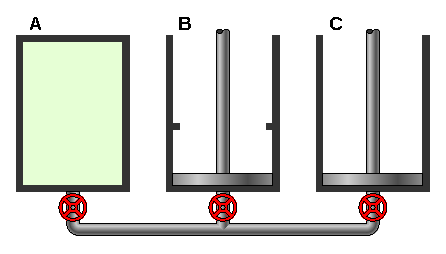
\includegraphics[scale=1.2]{resources/f04.eps}
\end{figure}

\textbf{\underline{Solución}:} \\

\underline{Datos provistos:}
\begin{equation*}
    \text{Freón 12 (R-12)}
\end{equation*}
\begin{equation*}
    V^a = 0.3[m^3]
\end{equation*}
\begin{equation*}
    V^b = V^c = 0
\end{equation*}
\begin{equation*}
    \text{Temperatura constante}
\end{equation*}
\begin{equation*}
    X_1^a = 1
\end{equation*}
\begin{equation*}
    P_1^a = 820[kPa]
\end{equation*}
\begin{equation*}
    P_1^b = 200[kPa]
\end{equation*}
\begin{equation*}
    A_E = 0.5[m^2]
\end{equation*}
\begin{equation*}
    d_E = 0.2[m]
\end{equation*}
\begin{equation*}
    P_1^c = 400[kPa]
\end{equation*}

\underline{Estado 1}: \\
De Tablas Termodinámicas se obtienen los valores para una presión aproximada a
$820[kPa]$:

\begin{equation*}
    P(0.84772[MPa]) = \begin{cases}
        T = 35^\circ C \\
        \nu_l = 0.000786[m^3/kg] & h_l = 69.551[kJ/kg] \\
        \nu_v = 0.020641[m^3/kg] & h_v = 201.446[kJ/kg] \\
    \end{cases}
\end{equation*}

Se halla la masa total a partir de su volumen especifico para un titulo de $1$:

\begin{equation*}
    m = \frac{V^a}{\nu_v} = \frac{0.3[m^3]}{0.020641[m^3/kg]}
      = 14.534[kg]
\end{equation*}

A partir de la entalpía, se halla la energía interna en el tanque $A$:

\begin{equation*}
    h = u + P\,\nu
\end{equation*}
\begin{equation*}
    \begin{split}
        u^a &= h_v - P^a\,\nu^a \\
            &= 201.446[kJ/kg] - (820[kPa]\,0.020641[m^3/kg]) \\
            &= 184.52[kJ/kg]
    \end{split}
\end{equation*}

\begin{figure}[H]
\centering
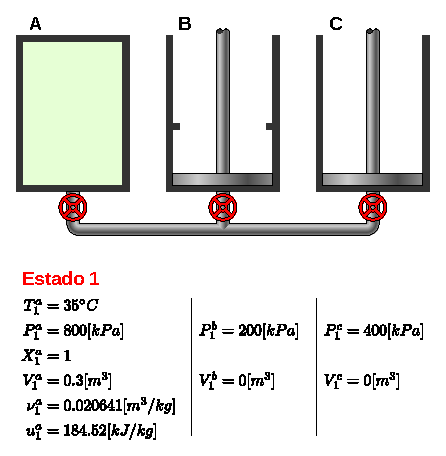
\includegraphics[scale=1.2]{resources/f04-1.eps}
\end{figure}

\underline{Estado 2}: \\
De Tablas Termodinámicas se obtienen los valores para una presión aproximada a
$400[kPa]$ y una temperatura de $35^\circ C$:

\begin{equation*}
    P(0.4[MPa])\,|\,T(40^\circ C) = \begin{cases}
        \nu = 0.050046[m^3/kg] \\
        h = 212.250[kJ/kg]
    \end{cases}
\end{equation*}

Se halla el volumen y energía interna de la combinación de todos los tanques
a partir del volumen especifico:

\begin{equation*}
    V = m\,\nu = 14.534[kg]\,0.050046[m^3/kg] = 0.7274[m^3]
\end{equation*}
\begin{equation*}
    \begin{split}
        u &= h - P\,\nu \\
          &= 212.250[kJ/kg] - (400[kPa]\,0.050046[m^3/kg]) \\
          &= 192.23[kJ/kg]
    \end{split}
\end{equation*}

Se halla la masa en cada tanque:

\begin{equation*}
    m^a = \frac{V^a}{\nu} = \frac{0.3[m^3]}{0.050046[m^3/kg]} = 5.9945[kg]
\end{equation*}
\begin{equation*}
    V^b = A_E\,d_E = 0.5[m^2]\,0.2[m] = 0.1[m^3]
\end{equation*}
\begin{equation*}
    m^b = \frac{V^b}{\nu} = \frac{0.1[m^3]}{0.050046[m^3/kg]} = 1.9982[kg]
\end{equation*}
\begin{equation*}
    V = V^a + V^b + V^c
\end{equation*}
\begin{equation*}
    V^c = V - V^a - V^b = 0.7274[m^3] - 0.3[m^3] - 0.1[m^3] = 0.3274[m^3]
\end{equation*}
\begin{equation*}
    m^c = \frac{V^c}{\nu} = \frac{0.3274[m^3]}{0.050046[m^3/kg]} = 6.5415[kg]
\end{equation*}

\begin{figure}[H]
\centering
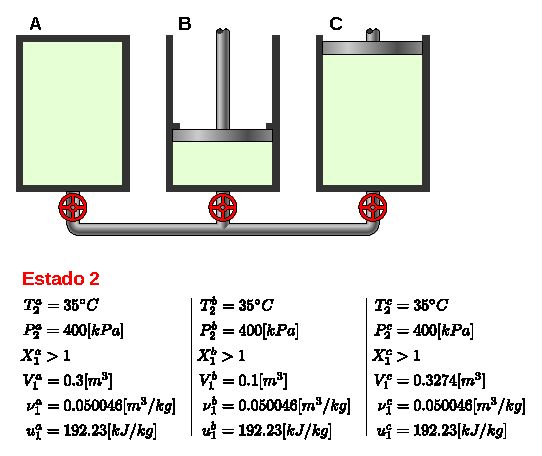
\includegraphics[scale=1.2]{resources/f04-2.eps}
\end{figure}

\underline{Trabajo}: \\
\begin{equation*}
    \begin{split}
    W_{1\rightarrow 2} &= W_{1\rightarrow 2}^a + W_{1\rightarrow 2}^b
                          + W_{1\rightarrow 2}^c \\
                       &= \int_1^2 P_{1\rightarrow 2}^a\,dv^a
                          + \int_1^2 P_{1\rightarrow 2}^b\,dv^b
                          + \int_1^2 P_{1\rightarrow 2}^c\,dv^c \\
                       &= 0 + P_{1\rightarrow 2}^b \int_1^2 dv^b
                          + P_{1\rightarrow 2}^c \int_1^2 dv^c \\
                       &= P_{1\rightarrow 2}^b (V_2^b - V_1^b)
                          + P_{1\rightarrow 2}^c (V_2^c - V_1^c) \\
                       &= 200[kPa](0.1[m^3]-0[m^3])
                          + 400[kPa](0.3274[m^3-0[m^3]) \\
                       &= 150.95[kJ]
    \end{split}
\end{equation*}

\underline{Calor}: \\
A partir de la primera ley de la termodinámica, se halla el calor intercambiado:

\begin{equation*}
    \Delta U_{1\rightarrow 2} = Q_{1\rightarrow 2} - W_{1\rightarrow 2}
\end{equation*}
\begin{equation*}
    \begin{split}
        Q_{1\rightarrow 2} &= \Delta U_{1\rightarrow 2} + W_{1\rightarrow 2} \\
                           &= (\Delta U^a_{1\rightarrow 2} 
                              + \Delta U^b_{1\rightarrow 2} 
                              + \Delta U^c_{1\rightarrow 2})
                              + W_{1\rightarrow 2} \\
                           &= (U_2^a - U_1^a + U_2^b - U_1^b + U_2^c - U_1^c)
                              + W_{1\rightarrow 2} \\
                           &= (U_2^a+U_2^b+U_2^c - (U_1^a+U_1^b+U_1^c))
                              + W_{1\rightarrow 2} \\
                           &= (m_2^a\,u_2^a+m_2^b\,u_2^b+m_2^c\,u_2^c
                              - (m_1^a\,u_1^a+m_1^b\,u_1^b+m_1^c\,u_1^c))
                              + W_{1\rightarrow 2} \\
                           &= (u_2\,(m_2^a+m_2^b+m_2^c)
                              - (m_1^a\,u_1^a+m_1^b\,u_1^b+m_1^c\,u_1^c))
                              + W_{1\rightarrow 2} \\
                           &= (u_2\,m-(m_1^a\,u_1^a+0+0))
                              + W_{1\rightarrow 2} \\
                           &= (u_2\,m-m\,u_1^a)+W_{1\rightarrow 2} \\
                           &= m\,(u_2-u_1^a)+W_{1\rightarrow 2} \\
                           &= 14.534[kg](192.23[kJ/kg]
                              -184.52[kJ/kg])+150.95[kJ] \\
                           &= 263.03[kJ]
    \end{split}
\end{equation*}

\begin{figure}[H]
\centering
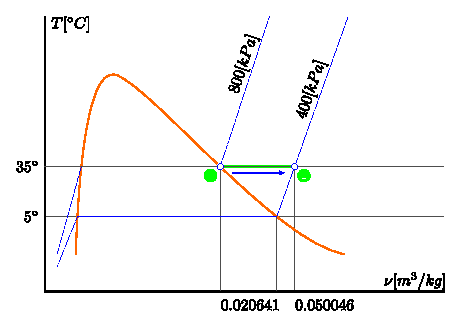
\includegraphics[scale=1.5]{resources/f04-d.eps}
\end{figure}

\begin{equation*}
\boxed{
    \begin{array}{l}
        Q = 263.03[kJ]
    \end{array}
}
\end{equation*}
\newpage

\item En un recipiente rígido de $5[m^3]$ esta contenida agua con un titulo de
$0.8$ y una presión de $2[MPa]$. Si la presión se reduce a $400[kPa]$ al
enfriarse el recipiente. Hallar las masas finales en estado liquido y de vapor;
también el calor intercambiado.

\begin{figure}[H]
\centering
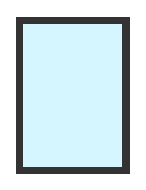
\includegraphics[scale=1.2]{resources/f05.eps}
\end{figure}

\textbf{\underline{Solución}:} \\

\underline{Datos provistos:}
\begin{equation*}
    \text{Agua}
\end{equation*}
\begin{equation*}
    V = 5[m^3]
\end{equation*}
\begin{equation*}
    X_1 = 0.8
\end{equation*}
\begin{equation*}
    P_1 = 2000[kPa]
\end{equation*}
\begin{equation*}
    P_2 = 400[kPa]
\end{equation*}

\underline{Estado 1}: \\
De Tablas Termodinámicas se obtienen los valores para una presión de
$2000[kPa]$:

\begin{equation*}
    P(2000[kPa]) = \begin{cases}
        T = 212.42^\circ C\\
        \nu_l = 0.001177[m^3/kg] & u_l = 906.42[kJ/kg] \\
        \nu_v = 0.09963[m^3/kg]  & u_v = 2600.26[kJ/kg]
    \end{cases}
\end{equation*}

Se halla el volumen especifico y energía interna a partir del titulo y los
valores de liquido y vapor:

\begin{equation*}
    \begin{split}
        \nu &= \nu_l + X_1(\nu_v - \nu_l) \\
            &= 0.001177 + 0.8 (0.09963 - 0.001177) \\
            &= 0.079939[m^3/kg]
    \end{split}
\end{equation*}
\begin{equation*}
    \begin{split}
        u &= u_l + X_1(u_v - u_l) \\
          &= 906.42 + 0.8 (2600.26 - 906.42) \\
          &= 2261.5[kJ/kg]
    \end{split}
\end{equation*}

Se halla la masa a partir de su volumen especifico:

\begin{equation*}
    m = \frac{V}{\nu} = \frac{5[m^3]}{0.079939[m^3/kg]}
      = 62.547[kg]
\end{equation*}

\begin{figure}[H]
\centering
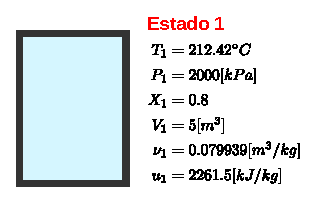
\includegraphics[scale=1.2]{resources/f05-1.eps}
\end{figure}

\underline{Estado 2}: \\
De Tablas Termodinámicas se obtienen los valores para una presión de
$400[kPa]$:

\begin{equation*}
    P(400[kPa]) = \begin{cases}
        T = 143.63^\circ C\\
        \nu_l = 0.001084[m^3/kg] & u_l = 604.29[kJ/kg] \\
        \nu_v = 0.46246[m^3/kg]  & u_v = 2553.55[kJ/kg]
    \end{cases}
\end{equation*}

El volumen especifico se mantiene constante:

\begin{equation*}
    \nu_2 = \nu_1 = 0.079939[m^3/kg]
\end{equation*}

Se halla el titulo a partir de su definición:

\begin{equation*}
    X = \frac{\nu-\nu_l}{\nu_v-\nu_l}
      = \frac{0.079939[m^3/kg] - 0.001084[m^3/kg]}
      {0.46246[m^3/kg] - 0.001084[m^3/kg]}
      = 0.1709
\end{equation*}

Se halla la energía interna a partir del titulo y los valores de liquido y
vapor:

\begin{equation*}
    \begin{split}
        u &= u_l + X_1(u_v - u_l) \\
          &= 604.29 + 0.1709 (2553.55 - 604.29) \\
          &= 937.44[kJ/kg]
    \end{split}
\end{equation*}

Se hallan las masas a partir de la definición de titulo:

\begin{equation*}
    X = \frac{m_v}{m}
\end{equation*}
\begin{equation*}
    m_v = X\,m = 0.1709\,62.547[kg] = 10.690[kg]
\end{equation*}
\begin{equation*}
    m_l + m_v = m
\end{equation*}
\begin{equation*}
    m_l = m - m_v = 62.547[kg] - 10.690[kg] = 51.857[kg]
\end{equation*}

\begin{figure}[H]
\centering
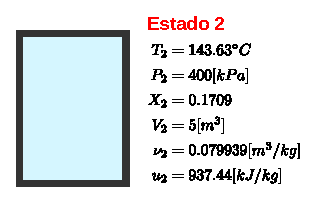
\includegraphics[scale=1.2]{resources/f05-2.eps}
\end{figure}

\underline{Trabajo}: \\
\begin{equation*}
    \begin{split}
    W_{1\rightarrow 2} &= \int_1^2 P_{1\rightarrow 2}\,dv \\
                       &= P_{1\rightarrow 2} \int_1^2 dv \\
                       &= P_{1\rightarrow 2} (V_2-V_1) \\
                       &= 0[kJ]
    \end{split}
\end{equation*}

\underline{Calor}: \\
A partir de la primera ley de la termodinámica, se halla el calor intercambiado:

\begin{equation*}
    \Delta U_{1\rightarrow 2} = Q_{1\rightarrow 2} - W_{1\rightarrow 2}
\end{equation*}
\begin{equation*}
    \begin{split}
        Q_{1\rightarrow 2} &= \Delta U_{1\rightarrow 2} + W_{1\rightarrow 2} \\
                           &= m(u_2 - u_1) + W_{1\rightarrow 2} \\
                           &= 62.547[kg](937.44[kJ/kg]-2261.5[kJ/kg])+0 \\
                           &= -82815.676[kJ]
    \end{split}
\end{equation*}

\begin{figure}[H]
\centering
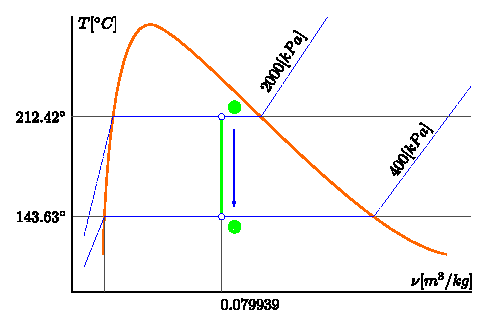
\includegraphics[scale=1.5]{resources/f05-d.eps}
\end{figure}

\begin{equation*}
\boxed{
    \begin{array}{l}
        Q = -82815.676[kJ]
    \end{array}
}
\end{equation*}
\newpage

\item Dentro un cilindro con su embolo se tiene $0.1[m^3]$ de agua saturada con
titulo del $25\%$ y una presión de $200[kPa]$. La masa del embolo es $40[kg]$ y
su diámetro $10[cm]$, la presión atmosférica de $1.3[kg/cm^2]$. Además sobre el
embolo hay un peso de que ejerce una presión de $120[kPa]$. Se entrega calor al
sistema hasta que su presión sea de $700[kPa]$ y su volumen de $0.2[m^3]$.
Hallar el calor intercambiado.

\begin{figure}[H]
\centering
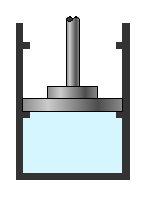
\includegraphics[scale=1.2]{resources/f06.eps}
\end{figure}

\textbf{\underline{Solución}:} \\

\underline{Datos provistos:}
\begin{equation*}
    \text{Agua}
\end{equation*}
\begin{equation*}
    V_1 = 0.1[m^3]
\end{equation*}
\begin{equation*}
    X_1 = 0.25
\end{equation*}
\begin{equation*}
    P_1 = 200[kPa]
\end{equation*}
\begin{equation*}
    m_E = 40[kg]
\end{equation*}
\begin{equation*}
    d_E = 0.1[m]
\end{equation*}
\begin{equation*}
    P_{atm} = 1.3[kg/cm^2]
\end{equation*}
\begin{equation*}
    P_P = 120[kPa]
\end{equation*}
\begin{equation*}
    P_4 = 700[kPa]
\end{equation*}
\begin{equation*}
    V_4 = 0.2[m^3]
\end{equation*}

\underline{Estado 1}: \\
De Tablas Termodinámicas se obtienen los valores para una presión de $200[kPa]$:

\begin{equation*}
    P(200[kPa]) = \begin{cases}
        T = 120.23^\circ C \\
        \nu_l = 0.001061[m^3/kg] & u_l = 504.47[kJ/kg] \\
        \nu_v = 0.88573[m^3/kg]  & u_v = 2529.49[kJ/kg]
    \end{cases}
\end{equation*}

Se calcula el volumen especifico y la energía interna para un titulo de $0.25$:

\begin{equation*}
    \begin{split}
        \nu &= \nu_l + X_1(\nu_v - \nu_l) \\
            &= 0.001061 + 0.25 (0.88573 - 0.001061) \\
            &= 0.2222[m^3/kg]
    \end{split}
\end{equation*}
\begin{equation*}
    \begin{split}
        u &= u_l + X_1(u_v - u_l) \\
          &= 504.47 + 0.25 (2529.49 - 504.47) \\
          &= 1010.7[kJ/kg]
    \end{split}
\end{equation*}

Se halla la masa a partir de su volumen especifico:

\begin{equation*}
    m = \frac{V}{\nu} = \frac{0.1[m^3]}{0.2222[m^3/kg]}
      = 0.45[kg]
\end{equation*}

\begin{figure}[H]
\centering
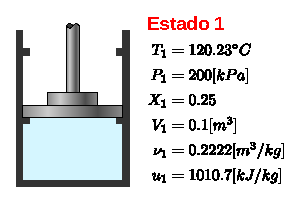
\includegraphics[scale=1.2]{resources/f06-1.eps}
\end{figure}

\underline{Estado 2}: \\
Se calcula la presión requerida para levantar el embolo:

\begin{equation*}
    \begin{split}
        P &= P_{atm} + P_E + P_P  \\
          &= P_{atm} + \frac{F_E}{A_E} + P_P \\
          &= P_{atm} + \frac{m_E\,g}{\pi r_E^2} + P_P \\
          &= 1.3[kg/cm^2]\frac{98[kPa]}{1[kg/cm^2]}
             + \frac{40[kg]\,9.8[m/s^2]}{\pi\,(0.05)^2[m^2]}
             \frac{1[kPa]}{1000[Pa]} + 120[kPa] \\
          &= 297.31[kPa]
    \end{split}
\end{equation*}

De Tablas Termodinámicas se obtienen los valores para una presión aproximada a
$297.31[kPa]$:

\begin{equation*}
    P(300[kPa]) = \begin{cases}
        T = 133.55^\circ C \\
        \nu_l = 0.001073[m^3/kg] & u_l = 561.13[kJ/kg] \\
        \nu_v = 0.60582[m^3/kg]  & u_v = 2543.55[kJ/kg]
    \end{cases}
\end{equation*}

Considerando que el proceso es a volumen constante, se halla el titulo:

\begin{equation*}
    X = \frac{\nu-\nu_l}{\nu_v-\nu_l}
      = \frac{0.2222[m^3/kg] - 0.001073[m^3/kg]}
      {0.60582[m^3/kg] - 0.001073[m^3/kg]}
      = 0.3657
\end{equation*}

\begin{figure}[H]
\centering
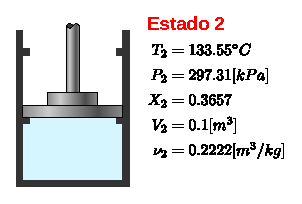
\includegraphics[scale=1.2]{resources/f06-2.eps}
\end{figure}

\underline{Estado 3}: \\
Se halla el volumen especifico a partir del volumen final y la masa:

\begin{equation*}
    \nu = \frac{V}{m} = \frac{0.2}{0.45} = 0.4445[m^3/kg]
\end{equation*}

\begin{figure}[H]
\centering
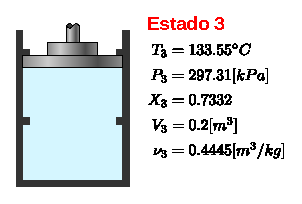
\includegraphics[scale=1.2]{resources/f06-3.eps}
\end{figure}

\underline{Estado 4}: \\
De Tablas Termodinámicas se obtienen los valores para una presión de $700[kPa]$:

\begin{equation*}
    P(700[kPa]) = \begin{cases}
        T = 164.97^\circ C \\
        \nu_l = 0.001108[m^3/kg] & u_l = 696.43[kJ/kg] \\
        \nu_v = 0.027286[m^3/kg] & u_v = 2572.49[kJ/kg]
    \end{cases}
\end{equation*}

Considerando que el volumen especifico de vapor es menor que el volumen
especifico actual ($\nu = 0.4445[m^3/kg]$), el agua se encuentra en la zona de
vapor sobrecalentado.

De Tablas Termodinámicas se obtienen los valores para una presión aproximada de
$700[kPa]$ y un volumen especifico de $0.4445[m^3/kg]$:

\begin{equation*}
    P(800[kPa])\,|\,\nu(0.44331[m^3/kg]) = \begin{cases}
        T = 500^\circ C \\
        u = 3125.95[kJ/kg]
    \end{cases}
\end{equation*}

\begin{figure}[H]
\centering
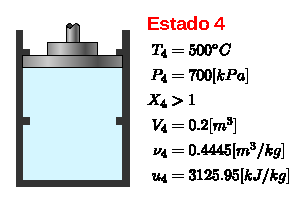
\includegraphics[scale=1.2]{resources/f06-4.eps}
\end{figure}

\underline{Trabajo}: \\
\begin{equation*}
    \begin{split}
    W_{1\rightarrow 4} &= W_{1\rightarrow 2} + W_{2\rightarrow 3}
                          + W_{3\rightarrow 4} \\
                       &= \int_1^2 P_{1\rightarrow 2}\,dv
                          + \int_2^3 P_{2\rightarrow 3}\,dv
                          + \int_3^4 P_{3\rightarrow 4}\,dv \\
                       &= 0 + P_2 \int_2^3 dv + 0 \\
                       &= P_2\,(V\Biggr|_2^3) \\
                       &= P_2(V_3-V_2) \\
                       &= 297.31[kPa](0.2[m^3]-0.1[m^3]) \\
                       &= 29.731[kJ]
    \end{split}
\end{equation*}

\underline{Calor}: \\
A partir de la primera ley de la termodinámica, se halla el calor intercambiado:

\begin{equation*}
    \Delta U_{1\rightarrow 4} = Q_{1\rightarrow 4} - W_{1\rightarrow 4}
\end{equation*}
\begin{equation*}
    \begin{split}
        Q_{1\rightarrow 4} &= \Delta U_{1\rightarrow 4} + W_{1\rightarrow 4} \\
                           &= m(u_4 - u_1) + W_{1\rightarrow 4} \\
                           &= 0.45[kg](3125.95[kJ/kg]
                              -1010.7[kJ/kg])+29.731[kJ] \\
                           &= 981.56[kJ]
    \end{split}
\end{equation*}

\begin{figure}[H]
\centering
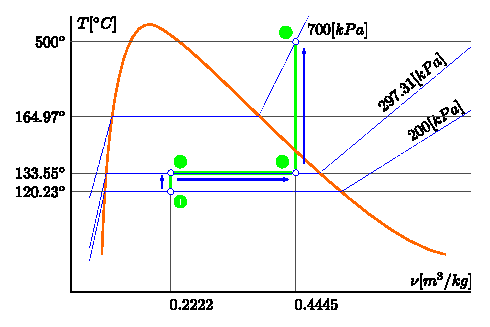
\includegraphics[scale=1.5]{resources/f06-d.eps}
\end{figure}

\begin{equation*}
\boxed{
    \begin{array}{l}
        Q = 981.56[kJ]
    \end{array}
}
\end{equation*}
\newpage

\item Según la figura se tiene dentro el cilindro con su embolo se tiene R-22
con una masa de $1[kg]$, $50^\circ C$ y $700[kPa]$. En esta posición el embolo
choca contra los topes. El sistema pierde calor hasta que llega al estado de
vapor saturado. En este estado la presión del sistema esta equilibrado con la
presión externa. El freón continua enfriándose hasta llegar al estado de liquido
saturado. Hallar el calor intercambiado.

\begin{figure}[H]
\centering
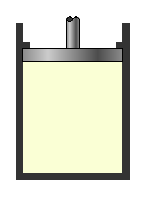
\includegraphics[scale=1.2]{resources/f07.eps}
\end{figure}

\textbf{\underline{Solución}:} \\

\underline{Datos provistos:}
\begin{equation*}
    \text{R-22}
\end{equation*}
\begin{equation*}
    m = 1[kg]
\end{equation*}
\begin{equation*}
    T_1 = 50^\circ C
\end{equation*}
\begin{equation*}
    P_1= 700[kPa]
\end{equation*}
\begin{equation*}
    X_2 = 1
\end{equation*}
\begin{equation*}
    P_2 = P_{atm}
\end{equation*}
\begin{equation*}
    X_3 = 0
\end{equation*}

\underline{Estado 1}: \\
De Tablas Termodinámicas se obtienen los valores para una presión de
$0.7[MPa]$ y una temperatura de $50^\circ C$:

\begin{equation*}
    P(0.8[MPa])\,|\,T(50^\circ C) = \begin{cases}
        \nu = 0.040763[m^3/kg] \\
        h = 283.282[kJ/kg]
    \end{cases}
\end{equation*}

Se halla el volumen a partir de la definición de volumen especifico:

\begin{equation*}
    V = \nu\,m = 0.040763[m^3/kg]\,1[kg] = 0.040763[m^3]
\end{equation*}

A partir de la entalpía, se halla la energía interna:

\begin{equation*}
    h = u + P\,\nu
\end{equation*}
\begin{equation*}
    \begin{split}
        u &= h - P\,\nu \\
            &= 283.282[kJ/kg] - (700[kPa]\,0.040763[m^3/kg]) \\
            &= 254.75[kJ/kg]
    \end{split}
\end{equation*}

\begin{figure}[H]
\centering
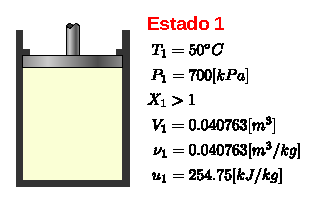
\includegraphics[scale=1.2]{resources/f07-1.eps}
\end{figure}

\underline{Estado 2}: \\
Considerando que la presión igualo a la presión externa, el proceso se realiza
a volumen constante:

\begin{equation*}
    \nu = 0.040763[m^3/kg]
\end{equation*}

De Tablas Termodinámicas se obtienen los valores para un volumen especifico
aproximado de $0.040763[m^3/kg]$ y un titulo de $1$:

\begin{equation*}
    \nu(0.040356[m^3/kg])\,|\,X(1) = \begin{cases}
        T = 5^\circ C \\
        P = 583.8[kPa]
    \end{cases}
\end{equation*}

\begin{figure}[H]
\centering
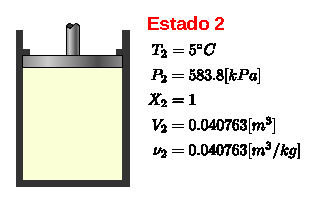
\includegraphics[scale=1.2]{resources/f07-2.eps}
\end{figure}

\underline{Estado 3}: \\
De Tablas Termodinámicas se obtienen los valores para una presión de
$583.8[kPa]$, una temperatura de $5^\circ C$ y un titulo de $0$:

\begin{equation*}
    P(0.5838[MPa])\,|\,T(5^\circ C)\,|\,X(0) = \begin{cases}
        \nu = 0.000789[m^3/kg] \\
        h = 50.485[kJ/kg]
    \end{cases}
\end{equation*}

Se halla el volumen a partir de la definición de volumen especifico:

\begin{equation*}
    V = \nu\,m = 0.000789[m^3/kg]\,1[kg] = 0.000789[m^3]
\end{equation*}

A partir de la entalpía, se halla la energía interna:

\begin{equation*}
    h = u + P\,\nu
\end{equation*}
\begin{equation*}
    \begin{split}
        u &= h - P\,\nu \\
            &= 50.485[kJ/kg] - (583.8[kPa]\,0.000789[m^3/kg]) \\
            &= 50.024[kJ/kg]
    \end{split}
\end{equation*}

\begin{figure}[H]
\centering
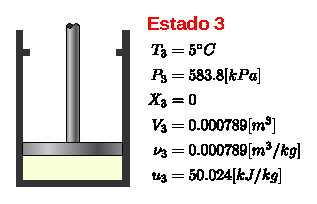
\includegraphics[scale=1.2]{resources/f07-3.eps}
\end{figure}

\underline{Trabajo}: \\
\begin{equation*}
    \begin{split}
    W_{1\rightarrow 3} &= W_{1\rightarrow 2} + W_{2\rightarrow 3} \\
                       &= \int_1^2 P_{1\rightarrow 2}\,dv
                          + \int_2^3 P_{2\rightarrow 3}\,dv \\
                       &= 0 + P_2 \int_2^3 dv \\
                       &= P_2\,(V\Biggr|_2^3) \\
                       &= P_2(V_3-V_2) \\
                       &= 583.8[kPa](0.000789[m^3]-0.040763[m^3]) \\
                       &= -23.337[kJ]
    \end{split}
\end{equation*}

\underline{Calor}: \\
A partir de la primera ley de la termodinámica, se halla el calor entregado:

\begin{equation*}
    \Delta U_{1\rightarrow 3} = Q_{1\rightarrow 3} - W_{1\rightarrow 3}
\end{equation*}
\begin{equation*}
    \begin{split}
        Q_{1\rightarrow 3} &= \Delta U_{1\rightarrow 3} + W_{1\rightarrow 3} \\
                           &= m(u_3 - u_1) + W_{1\rightarrow 3} \\
                           &= 1[kg](50.024[kJ/kg]-254.75[kJ/kg])-23.337[kJ] \\
                           &= -228.06[kJ]
    \end{split}
\end{equation*}

\begin{figure}[H]
\centering
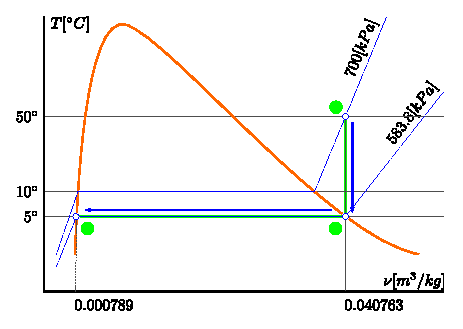
\includegraphics[scale=1.5]{resources/f07-d.eps}
\end{figure}

\begin{equation*}
\boxed{
    \begin{array}{l}
        Q = -228.06[kJ]
    \end{array}
}
\end{equation*}
\newpage

\item Según la figura el tanque $A$ tiene un volumen de $0.2[m^3]$ y contiene
freón 12 como vapor saturado a $30^\circ C$, cuando se abren las válvulas el
freón entra al cilindro $B$ en el cual se tiene un embolo que requiere una
presión de $0.14[MPa]$ para ser elevado. En el tanque $C$ que tiene un volumen
de $40[lt]$ también tiene freón a $0.74[MPa]$ como liquido saturado. El proceso
termina cuando los 3 elementos se equilibran en presión y su temperatura final
es de $30^\circ C$. Hallar las masas finales en cada recipiente el calor
entregado y el trabajo realizado.

\begin{figure}[H]
\centering
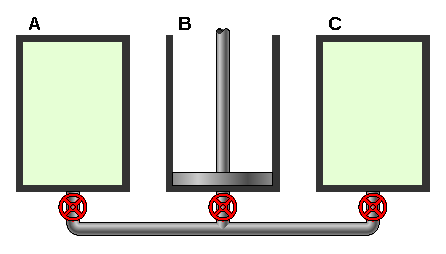
\includegraphics[scale=1.2]{resources/f08.eps}
\end{figure}

\textbf{\underline{Solución}:} \\

\underline{Datos provistos:}
\begin{equation*}
    \text{Freón 12 (R-12)}
\end{equation*}
\begin{equation*}
    V^a = 0.2[m^3]
\end{equation*}
\begin{equation*}
    V^c = 40[lt]\frac{0.001[m^3]}{1[lt]}=0.04[m^3]
\end{equation*}
\begin{equation*}
    X_1^a = 1
\end{equation*}
\begin{equation*}
    T_1^a = 30^\circ C
\end{equation*}
\begin{equation*}
    P_1^b = 0.14[MPa]
\end{equation*}
\begin{equation*}
    P_1^c = 0.74[MPa]
\end{equation*}
\begin{equation*}
    X_1^c = 0
\end{equation*}
\begin{equation*}
    T_2 = 30^\circ C
\end{equation*}

\underline{Estado 1}: \\
De Tablas Termodinámicas se obtienen los valores para una temperatura
de $30^\circ C$ y un titulo de $1$ en el tanque $A$:

\begin{equation*}
    T(30^\circ C)\,|\,X(1) = \begin{cases}
        P = 0.74490[MPa] \\
        \nu = 0.023508[m^3/kg] \\
        h = 199.620[kJ/kg]
    \end{cases}
\end{equation*}

Se halla la masa a partir de su volumen especifico:

\begin{equation*}
    m^a = \frac{V^a}{\nu} = \frac{0.2[m^3]}{0.023508[m^3/kg]}
      = 8.5077[kg]
\end{equation*}

A partir de la entalpía, se halla la energía interna:

\begin{equation*}
    h = u + P\,\nu
\end{equation*}
\begin{equation*}
    \begin{split}
        u^a &= h - P^a\,\nu^a \\
            &= 199.620[kJ/kg] - (744.90[kPa]\,0.023508[m^3/kg]) \\
            &= 182.11[kJ/kg]
    \end{split}
\end{equation*}

De Tablas Termodinámicas se obtienen los valores para una presión aproximada
de $0.74[MPa]$ y un titulo de $0$ en el tanque $C$:

\begin{equation*}
    P(0.74[MPa])\,|\,X(0) = \begin{cases}
        T = 30^\circ C \\
        \nu = 0.000774[m^3/kg] \\
        h = 64.592[kJ/kg]
    \end{cases}
\end{equation*}

Se halla la masa a partir de su volumen especifico:

\begin{equation*}
    m^c = \frac{V^c}{\nu} = \frac{0.04[m^3]}{0.000774[m^3/kg]}
      = 51.68[kg]
\end{equation*}

A partir de la entalpía, se halla la energía interna:

\begin{equation*}
    h = u + P\,\nu
\end{equation*}
\begin{equation*}
    \begin{split}
        u^c &= h - P^c\,\nu^c \\
            &= 64.592[kJ/kg] - (744.90[kPa]\,0.000774[m^3/kg]) \\
            &= 64.015[kJ/kg]
    \end{split}
\end{equation*}

Se halla la masa total a partir de las masas en $A$, $B$ y $C$:

\begin{equation*}
    \begin{split}
        m &= m^a + m^b + m^c \\
          &= 8.5077[kg] + 0[kg] + 51.68[kg] \\
          &= 60.187[kg]
    \end{split}
\end{equation*}

\begin{figure}[H]
\centering
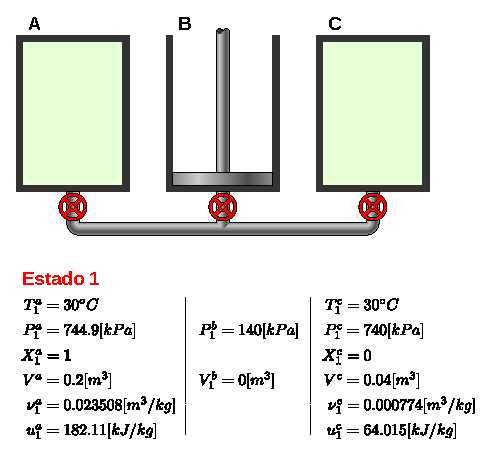
\includegraphics[scale=1.2]{resources/f08-1.eps}
\end{figure}

\underline{Estado 2}: \\
De Tablas Termodinámicas se obtienen los valores para una presión aproximada de
$0.14[MPa]$ y una temperatura de $30^\circ C$:

\begin{equation*}
    P(0.15[MPa])\,|\,T(30^\circ C) = \begin{cases}
        \nu = 0.135000[m^3/kg] \\
        h = 209.314[kJ/kg]
    \end{cases}
\end{equation*}

Se halla el volumen total, y el volumen del tanque $B$ a partir de la definición
de volumen especifico:

\begin{equation*}
    V = \nu\,m = (0.135000[m^3/kg])(60.187[kg]) = 8.1253[m^3]
\end{equation*}
\begin{equation*}
    V^a + V^b + V^c = V
\end{equation*}
\begin{equation*}
    V^b = V - V^a - V^b = 8.1253[m^3] - 0.2[m^3] - 0.04[m^3] = 7.8853[m^3]
\end{equation*}

A partir de la entalpía, se halla la energía interna:

\begin{equation*}
    h = u + P\,\nu
\end{equation*}
\begin{equation*}
    \begin{split}
        u &= h - P\,\nu \\
          &= 209.314[kJ/kg] - (140[kPa]\,0.135000[m^3/kg]) \\
          &= 190.41[kJ/kg]
    \end{split}
\end{equation*}

Por tanto las masas resultantes son:

\begin{equation*}
    m^a = \frac{V^a}{\nu} = \frac{0.2}{0.135000} = 1.4815[kg]
\end{equation*}
\begin{equation*}
    m^b = \frac{V^b}{\nu} = \frac{7.8853}{0.135000} = 58.410[kg]
\end{equation*}
\begin{equation*}
    m^c = \frac{V^c}{\nu} = \frac{0.04}{0.135000} = 0.2963[kg]
\end{equation*}

\begin{figure}[H]
\centering
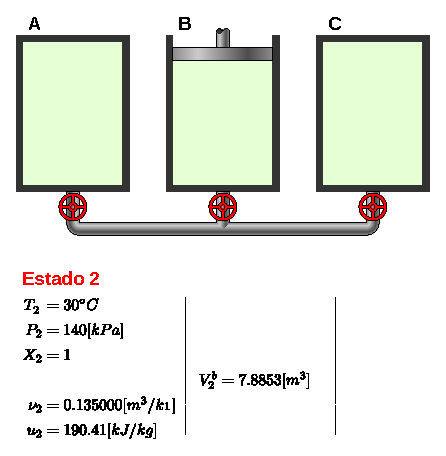
\includegraphics[scale=1.2]{resources/f08-2.eps}
\end{figure}

\underline{Trabajo}: \\
\begin{equation*}
    \begin{split}
    W_{1\rightarrow 2} &= W_{1\rightarrow 2}^a + W_{1\rightarrow 2}^b
                          + W_{1\rightarrow 2}^c \\
                       &= \int_1^2 P_{1\rightarrow 2}^a\,dv^a
                          + \int_1^2 P_{1\rightarrow 2}^b\,dv^b
                          + \int_1^2 P_{1\rightarrow 2}^c\,dv^c \\
                       &= 0 + P_{1\rightarrow 2}^b \int_1^2 dv^b + 0 \\
                       &= P_{1\rightarrow 2}^b (V_2^b - V_1^b) \\
                       &= 140[kPa](58.410[m^3]-0[m^3]) \\
                       &= 8177.3[kJ]
    \end{split}
\end{equation*}

\underline{Calor}: \\
A partir de la primera ley de la termodinámica, se halla el calor intercambiado:

\begin{equation*}
    \Delta U_{1\rightarrow 2} = Q_{1\rightarrow 2} - W_{1\rightarrow 2}
\end{equation*}
\begin{equation*}
    \begin{split}
        Q_{1\rightarrow 2} &= \Delta U_{1\rightarrow 2} + W_{1\rightarrow 2} \\
                           &= (\Delta U^a_{1\rightarrow 2} 
                              + \Delta U^b_{1\rightarrow 2} 
                              + \Delta U^c_{1\rightarrow 2})
                              + W_{1\rightarrow 2} \\
                           &= (U_2^a - U_1^a + U_2^b - U_1^b + U_2^c - U_1^c)
                              + W_{1\rightarrow 2} \\
                           &= (U_2^a+U_2^b+U_2^c - (U_1^a+U_1^b+U_1^c))
                              + W_{1\rightarrow 2} \\
                           &= (m_2^a\,u_2^a+m_2^b\,u_2^b+m_2^c\,u_2^c
                              - (m_1^a\,u_1^a+m_1^b\,u_1^b+m_1^c\,u_1^c))
                              + W_{1\rightarrow 2} \\
                           &= (u_2\,(m_2^a+m_2^b+m_2^c)
                              - (m_1^a\,u_1^a+m_1^b\,u_1^b+m_1^c\,u_1^c))
                              + W_{1\rightarrow 2} \\
                           &= (u_2\,m-(m_1^a\,u_1^a+0+m_1^c\,u_1^c))
                              + W_{1\rightarrow 2} \\
                           &= (u_2\,m-m_1^a\,u_1^a-m_1^c\,u_1^c)
                              + W_{1\rightarrow 2} \\
                           &= 60.187[kg]190.41[kJ/kg]-8.5077[kg]182.11[kJ/kg]
                              - 51.68[kg]64.015[kJ/kg] \\
                           &+ 8177.3[kJ] \\
                           &= 14780.220[kJ]
    \end{split}
\end{equation*}

\begin{figure}[H]
\centering
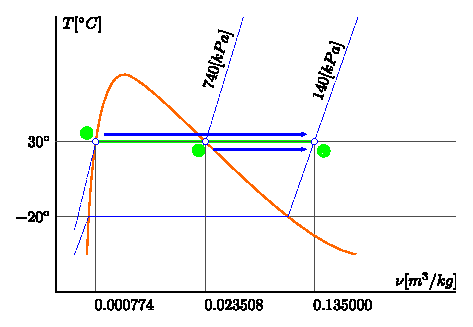
\includegraphics[scale=1.5]{resources/f08-d.eps}
\end{figure}

\begin{equation*}
\boxed{
    \begin{array}{l}
        m^a = 1.4815[kg] \\
        m^b = 58.410[kg] \\
        m^c = 0.2963[kg] \\
        W = 8177.3[kJ] \\
        Q = 14780.220[kJ]
    \end{array}
}
\end{equation*}
\newpage

\item Considere el esquema de la figura. El tanque $A$ tiene un volumen de
$100[lt]$ y contiene vapor saturado de R-134a a $30^\circ C$. El cilindro $B$
inicialmente esta vacío. Se abre la válvula y el refrigerante fluye al cilindro
$B$. La presión para elevar el embolo es de $200[kPa]$. Se entrega calor de modo
que la temperatura este siempre a $30^\circ C$. El proceso termina cuando se
alcanza un estado uniforme en $A$ y en $B$. Hallar las masas finales en cada
recipiente, el trabajo realizado y el calor intercambiado.

\begin{figure}[H]
\centering
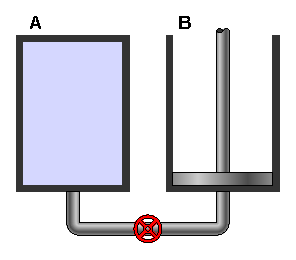
\includegraphics[scale=1.2]{resources/f09.eps}
\end{figure}

\textbf{\underline{Solución}:} \\

\underline{Datos provistos:}
\begin{equation*}
    \text{R-134a}
\end{equation*}
\begin{equation*}
    \text{Temperatura constante}
\end{equation*}
\begin{equation*}
    V^a = 100[lt]\frac{0.001[m^3]}{1[lt]} = 0.1[m^3]
\end{equation*}
\begin{equation*}
    X_1^a = 1
\end{equation*}
\begin{equation*}
    T_1^a = 30^\circ C
\end{equation*}
\begin{equation*}
    V_1^b = 0[m^3]
\end{equation*}
\begin{equation*}
    P_2 = 200[kPa]
\end{equation*}

\underline{Estado 1}: \\
De Tablas Termodinámicas se obtienen los valores para una temperatura
$30^\circ C$ y un titulo de $1$:

\begin{equation*}
    T(30^\circ C])\,|\,X(1) = \begin{cases}
        P = 771.0[kPa] \\
        \nu = 0.02671[m^3/kg] \\
        u = 394.48[kJ/kg]
    \end{cases}
\end{equation*}

Se halla la masa a partir de su volumen especifico:

\begin{equation*}
    m^a = \frac{V^a}{\nu} = \frac{0.1[m^3]}{0.02671[m^3/kg]}
      = 3.7439[kg]
\end{equation*}

\begin{figure}[H]
\centering
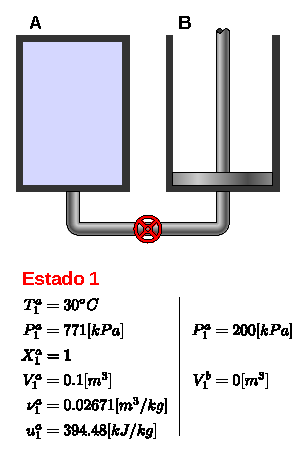
\includegraphics[scale=1.2]{resources/f09-1.eps}
\end{figure}

\underline{Estado 2}: \\
De Tablas Termodinámicas se obtienen los valores para una temperatura
$30^\circ C$ y una presión de $200[kPa]$:

\begin{equation*}
    T(30^\circ C)\,|\,P(200[kPa]) = \begin{cases}
        \nu = 0.11889[m^3/kg] \\
        u = 403.10[kJ/kg]
    \end{cases}
\end{equation*}

Se halla la masa en cada tanque a partir del volumen especifico:

\begin{equation*}
    m^a = \frac{V^a}{\nu} = \frac{0.1[m^3]}{0.11889[m^3/kg]}
      = 0.8411[kg]
\end{equation*}
\begin{equation*}
    m^a + m^b = m
\end{equation*}
\begin{equation*}
    m^b = m - m^a = 3.7439[kg] - 0.8411[kg] = 2.9028[kg]
\end{equation*}

Se halla el volumen en el tanque $B$:

\begin{equation*}
    V^b = m^b\,\nu = 2.9028[kg]\,0.11889[m^3/kg] = 0.3451[m^3]
\end{equation*}

\begin{figure}[H]
\centering
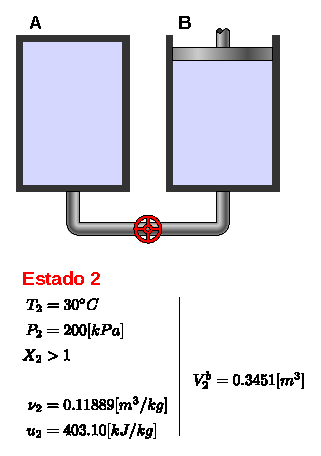
\includegraphics[scale=1.2]{resources/f09-2.eps}
\end{figure}

\underline{Trabajo}: \\
\begin{equation*}
    \begin{split}
    W_{1\rightarrow 2} &= W_{1\rightarrow 2}^a + W_{1\rightarrow 2}^b \\
                       &= \int_1^2 P_{1\rightarrow 2}^a\,dv^a
                          + \int_1^2 P_{1\rightarrow 2}^b\,dv^b \\
                       &= 0 + P_{1\rightarrow 2}^b \int_1^2 dv^b \\
                       &= P_{1\rightarrow 2}^b (V_2^b - V_1^b) \\
                       &= 200[kPa](0.3451[m^3]-0[m^3]) \\
                       &= 69.023[kJ]
    \end{split}
\end{equation*}

\underline{Calor}: \\
A partir de la primera ley de la termodinámica, se halla el calor intercambiado:

\begin{equation*}
    \Delta U_{1\rightarrow 2} = Q_{1\rightarrow 2} - W_{1\rightarrow 2}
\end{equation*}
\begin{equation*}
    \begin{split}
        Q_{1\rightarrow 2} &= \Delta U_{1\rightarrow 2} + W_{1\rightarrow 2} \\
                           &= (\Delta U^a_{1\rightarrow 2} 
                              + \Delta U^b_{1\rightarrow 2})
                              + W_{1\rightarrow 2} \\
                           &= (U_2^a - U_1^a + U_2^b - U_1^b)
                              + W_{1\rightarrow 2} \\
                           &= (U_2^a+U_2^b - (U_1^a+U_1^b))
                              + W_{1\rightarrow 2} \\
                           &= (m_2^a\,u_2^a+m_2^b\,u_2^b
                              - (m_1^a\,u_1^a+m_1^b\,u_1^b))
                              + W_{1\rightarrow 2} \\
                           &= (u_2\,(m_2^a+m_2^b)
                              - (m_1^a\,u_1^a+m_1^b\,u_1^b))
                              + W_{1\rightarrow 2} \\
                           &= (u_2\,m-(m_1^a\,u_1^a+0))
                              + W_{1\rightarrow 2} \\
                           &= (u_2\,m-m\,u_1^a)+W_{1\rightarrow 2} \\
                           &= m\,(u_2-u_1^a)+W_{1\rightarrow 2} \\
                           &= 3.7439[kg](403.10[kJ/kg]
                              -394.48[kJ/kg])+69.023[kJ] \\
                           &= 101.30[kJ]
    \end{split}
\end{equation*}

\begin{figure}[H]
\centering
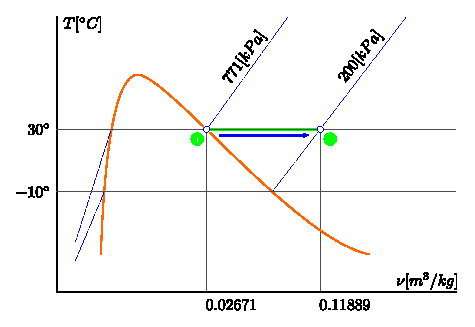
\includegraphics[scale=1.5]{resources/f09-d.eps}
\end{figure}

\begin{equation*}
\boxed{
    \begin{array}{l}
        m^a = 0.8411[kg] \\
        m^b = 2.9028[kg] \\
        W = 69.023[kJ] \\
        Q = 101.30[kJ]
    \end{array}
}
\end{equation*}
\newpage

\item Según la figura el tanque $A$ tiene un volumen de $1[m^3]$ y contiene
vapor saturado a $100[kPa]$; el cilindro $B$ también de $1[m^3]$ contiene agua a
$400^\circ C$ y $300[kPa]$. Se abre la válvula y se espera que el sistema
alcance el estado de equilibrio a los $200^\circ C$. Hallar las masas finales en
cada recipiente y el calor intercambiado.

\begin{figure}[H]
\centering
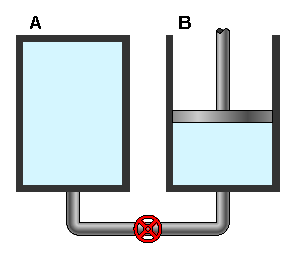
\includegraphics[scale=1.2]{resources/f10.eps}
\end{figure}

\textbf{\underline{Solución}:} \\

\underline{Datos provistos:}
\begin{equation*}
    \text{Agua}
\end{equation*}
\begin{equation*}
    V_1^a = 1[m^3]
\end{equation*}
\begin{equation*}
    X_1^a = 1
\end{equation*}
\begin{equation*}
    P_1^a = 100[kPa]
\end{equation*}
\begin{equation*}
    V_1^b = 1[m^3]
\end{equation*}
\begin{equation*}
    T_1^b = 400^\circ C
\end{equation*}
\begin{equation*}
    P_1^b = 300[kPa]
\end{equation*}
\begin{equation*}
    T_2 = 200^\circ C
\end{equation*}
\begin{equation*}
    P_2 = 300[kPa]
\end{equation*}

\underline{Estado 1}: \\
De Tablas Termodinámicas se obtienen los valores para una presión de
$100[kPa]$ y un titulo de $1$ para el tanque $A$:

\begin{equation*}
    P(100[kPa])\,|\,X(1) = \begin{cases}
        T = 99.62^\circ C \\
        \nu = 1.69400[m^3/kg] \\
        u = 2506.06[kJ/kg]
    \end{cases}
\end{equation*}

Se halla la masa a partir de su volumen especifico del tanque $A$:

\begin{equation*}
    m^a = \frac{V^a}{\nu} = \frac{1[m^3]}{1.69400[m^3/kg]}
      = 0.5903[kg]
\end{equation*}

De Tablas Termodinámicas se obtienen los valores para una temperatura de
$400^\circ C$ y la presión de $300[kPa]$ para el tanque $B$:

\begin{equation*}
    P(300[kPa])\,|\,T(400^\circ C) = \begin{cases}
        \nu = 1.03151[m^3/kg] \\
        u = 2965.53[kJ/kg]
    \end{cases}
\end{equation*}

Se halla la masa a partir de su volumen especifico del tanque $B$:

\begin{equation*}
    m^b = \frac{V^b}{\nu} = \frac{1[m^3]}{1.03151[m^3/kg]}
      = 0.9695[kg]
\end{equation*}

La masa total del sistema resulta:

\begin{equation*}
    m = m^a + m^b = 0.5903[kg] + 0.9695[kg] = 1.5598[kg]
\end{equation*}

\begin{figure}[H]
\centering
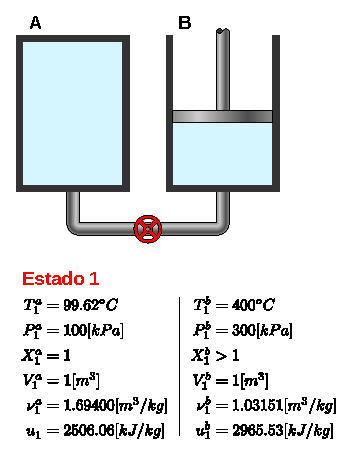
\includegraphics[scale=1.2]{resources/f10-1.eps}
\end{figure}

\underline{Estado 2}: \\
De Tablas Termodinámicas se obtienen los valores para una presión aproximada de
$300[kPa]$ y una temperatura de $200^\circ C$:

\begin{equation*}
    P(300[kPa])\,|\,T(200^\circ C) = \begin{cases}
        \nu = 0.71629[m^3/kg] \\
        u = 2650.65[kJ/kg]
    \end{cases}
\end{equation*}

Se halla el volumen total a partir de la definición de volumen especifico:

\begin{equation*}
    V = \nu\,m = 0.71629[m^3/kg]\,1.5598[kg] = 1.1172[m^3]
\end{equation*}
\begin{equation*}
    V^b = V - V^a = 1.1172[m^3] - 1[m^3] = 0.1172[m^3]
\end{equation*}

Por tanto las masas resultantes son:

\begin{equation*}
    m^a = \frac{V^a}{\nu} = \frac{1}{0.71629} = 1.3960[kg]
\end{equation*}
\begin{equation*}
    m^b = \frac{V^b}{\nu} = \frac{0.1172}{0.71629} = 0.1637[kg]
\end{equation*}

\begin{figure}[H]
\centering
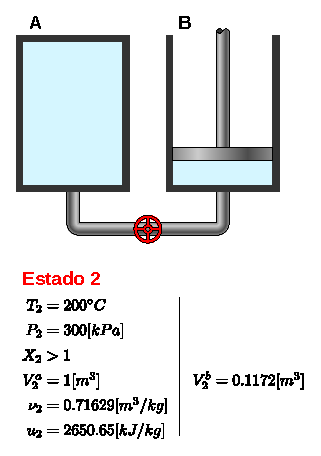
\includegraphics[scale=1.2]{resources/f10-2.eps}
\end{figure}

\underline{Trabajo}: \\
\begin{equation*}
    \begin{split}
    W_{1\rightarrow 2} &= W_{1\rightarrow 2}^a + W_{1\rightarrow 2}^b \\
                       &= \int_1^2 P_{1\rightarrow 2}^a\,dv^a
                          + \int_1^2 P_{1\rightarrow 2}^b\,dv^b \\
                       &= 0 + P_{1\rightarrow 2}^b \int_1^2 dv^b \\
                       &= P_{1\rightarrow 2}^b (V_2^b - V_1^b) \\
                       &= 300[kPa](0.1172[m^3]-1[m^3]) \\
                       &= -264.83[kJ]
    \end{split}
\end{equation*}

\underline{Calor}: \\
A partir de la primera ley de la termodinámica, se halla el calor intercambiado:

\begin{equation*}
    \Delta U_{1\rightarrow 2} = Q_{1\rightarrow 2} - W_{1\rightarrow 2}
\end{equation*}
\begin{equation*}
    \begin{split}
        Q_{1\rightarrow 2} &= \Delta U_{1\rightarrow 2} + W_{1\rightarrow 2} \\
                           &= (\Delta U^a_{1\rightarrow 2} 
                              + \Delta U^b_{1\rightarrow 2})
                              + W_{1\rightarrow 2} \\
                           &= (U_2^a - U_1^a + U_2^b - U_1^b)
                              + W_{1\rightarrow 2} \\
                           &= (U_2^a+U_2^b - (U_1^a+U_1^b))
                              + W_{1\rightarrow 2} \\
                           &= (m_2^a\,u_2^a+m_2^b\,u_2^b
                              - (m_1^a\,u_1^a+m_1^b\,u_1^b))
                              + W_{1\rightarrow 2} \\
                           &= (u_2\,(m_2^a+m_2^b)
                              - (m_1^a\,u_1^a+m_1^b\,u_1^b))
                              + W_{1\rightarrow 2} \\
                           &= (u_2\,m-(m_1^a\,u_1^a+m_1^b\,u_1^b))
                              + W_{1\rightarrow 2} \\
                           &= 1.5597[kg]2650.65[kJ/kg]
                              - 0.5903[kg]2506.06[kJ/kg] \\
                           &- 0.9694[kg]2965.53[kJ/kg]-264.83[kJ] \\
                           &= -484.73[kJ]
    \end{split}
\end{equation*}

\begin{figure}[H]
\centering
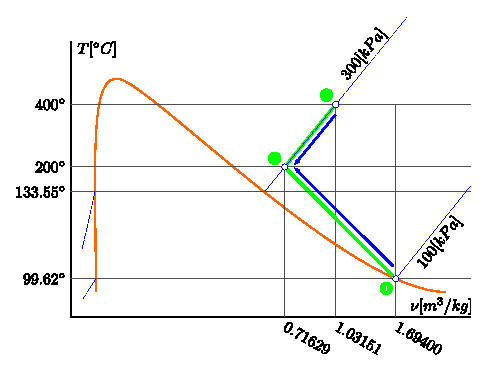
\includegraphics[scale=1.5]{resources/f10-d.eps}
\end{figure}

\begin{equation*}
\boxed{
    \begin{array}{l}
        m^a = 1.3960[kg] \\
        m^b = 0.1637[kg] \\
        W = -264.83[kJ] \\
        Q = -484.73[kJ]
    \end{array}
}
\end{equation*}
\newpage

\item Considere los 2 tanques conectados por una válvula conteniendo agua. El
volumen de $A$ es de $1[m^3]$ y el agua esta a $200[kPa]$ y $\nu=0.5[m^3/kg]$.
El tanque $B$ contiene $3.5[kg]$ de agua a $0.5[MPa]$ y $400^\circ C$. Se abre
la válvula hasta que se llega al estado de equilibrio. Hallar el volumen
especifico en el estado final.

\begin{figure}[H]
\centering
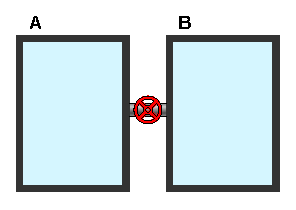
\includegraphics[scale=1.2]{resources/f11.eps}
\end{figure}

\textbf{\underline{Solución}:} \\

\underline{Datos provistos:}
\begin{equation*}
    \text{Agua}
\end{equation*}
\begin{equation*}
    V_1^a = 1[m^3]
\end{equation*}
\begin{equation*}
    P_1^a = 200[kPa]
\end{equation*}
\begin{equation*}
    \nu_1^a = 0.5[m^3/kg]
\end{equation*}
\begin{equation*}
    m_1^b = 3.5[kg]
\end{equation*}
\begin{equation*}
    P_1^b = 500[kPa]
\end{equation*}
\begin{equation*}
    T_1^b = 400^\circ C
\end{equation*}

\underline{Estado 1}: \\
De Tablas Termodinámicas se obtienen los valores para una presión de
$200[kPa]$ para el tanque $A$:

\begin{equation*}
    P(200[kPa]) = \begin{cases}
        T = 120.23^\circ C \\
        \nu_l = 0.001061[m^3/kg] \\
        \nu_v = 0.88573[m^3/kg]
    \end{cases}
\end{equation*}

Se halla el titulo a partir de su definición:

\begin{equation*}
    X^a = \frac{\nu-\nu_l}{\nu_v-\nu_l}
        = \frac{0.5[m^3/kg] - 0.001061[m^3/kg]}
          {0.88573[m^3/kg] - 0.001061[m^3/kg]}
        = 0.5640
\end{equation*}

Se halla la masa a partir de su volumen especifico:

\begin{equation*}
    m^a = \frac{V^a}{\nu} = \frac{1[m^3]}{0.5[m^3/kg]}
        = 2[kg]
\end{equation*}

De Tablas Termodinámicas se obtienen los valores para una presión de
$500[kPa]$ y una temperatura de $400^\circ C$ para el tanque $B$:

\begin{equation*}
    P(500[kPa])\,|\,T(400^\circ C) = \begin{cases}
        \nu = 0.61728[m^3/kg]
    \end{cases}
\end{equation*}

Se halla el volumen a partir de la definición de volumen especifico:

\begin{equation*}
    V^b = \nu\,m = 0.61728[m^3/kg]3.5[kg] = 2.1605[m^3]
\end{equation*}

\begin{figure}[H]
\centering
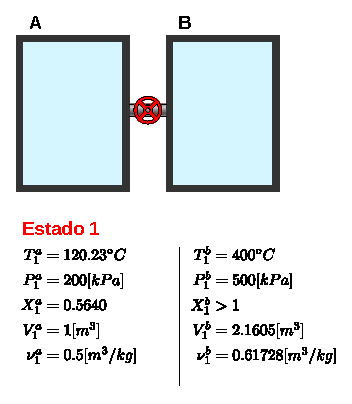
\includegraphics[scale=1.2]{resources/f11-1.eps}
\end{figure}

\underline{Estado 2}: \\
Se halla el volumen especifico a partir de su definición:

\begin{equation*}
    \nu = \frac{V_1^a+V_1^b}{m^a+m^b}
        = \frac{1[m^3]+2.1605[m^3]}{3.5[kg]+2[kg]}
        = 0.5746[m^3/kg]
\end{equation*}

\begin{figure}[H]
\centering
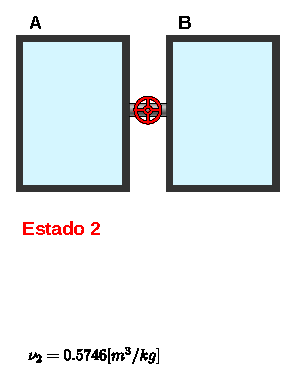
\includegraphics[scale=1.2]{resources/f11-2.eps}
\end{figure}

\begin{figure}[H]
\centering
\includegraphics[scale=1.5]{resources/f11-d.eps}
\end{figure}

\begin{equation*}
\boxed{
    \begin{array}{l}
        \nu = 0.5746[m^3/kg]
    \end{array}
}
\end{equation*}
\newpage

\item Según la figura se tiene $3[kg]$ de agua como liquido saturado a
$200[kPa]$. Se transfiere calor hasta que el embolo alcance los topes donde el
volumen es de $60[lt]$. Se continua entregando mas calor hasta que se duplica la
presión. Hallar la temperatura cuando el embolo alcanza los topes, el trabajo
realizado y el calor intercambiado.

\begin{figure}[H]
\centering
\includegraphics[scale=1.2]{resources/f12.eps}
\end{figure}

\textbf{\underline{Solución}:} \\

\underline{Datos provistos:}
\begin{equation*}
    \text{Agua}
\end{equation*}
\begin{equation*}
    m = 3[kg]
\end{equation*}
\begin{equation*}
    X_1 = 0
\end{equation*}
\begin{equation*}
    P_1 = 200[kPa]
\end{equation*}
\begin{equation*}
    V_2 = 60[lt]\frac{0.001[m^3]}{1[lt]} = 0.06[m^3]
\end{equation*}
\begin{equation*}
    P_2 = 200[kPa]
\end{equation*}
\begin{equation*}
    P_3 = 2\,P_2 = 400[kPa]
\end{equation*}

\underline{Estado 1}: \\
De Tablas Termodinámicas se obtienen los valores para una presión de
$200[kPa]$ y un titulo de $0$:

\begin{equation*}
    P(200[kPa])\,|\,X(0) = \begin{cases}
        T = 120.23^\circ C \\
        \nu = 0.001061[m^3/kg] \\
        u = 504.47[kJ/kg]
    \end{cases}
\end{equation*}

Se halla el volumen a partir de la definición de volumen especifico:

\begin{equation*}
    V = \nu\,m = 0.001061[m^3/kg]\,3[kg] = 0.003[m^3]
\end{equation*}

\begin{figure}[H]
\centering
\includegraphics[scale=1.2]{resources/f12-1.eps}
\end{figure}

\underline{Estado 2}: \\
Se halla el volumen especifico a partir de su definición:

\begin{equation*}
    \nu = \frac{V}{m} = \frac{0.06[m^3]}{3[kg]} = 0.02[m^3/kg]
\end{equation*}

De Tablas Termodinámicas se obtienen los valores para una presión de $200[kPa]$:

\begin{equation*}
    P(200[kPa])\,|\,T(120.23^\circ C) = \begin{cases}
        \nu_l = 0.001061[m^3/kg] & u_l = 504.47[kJ/kg] \\
        \nu_v = 0.88573[m^3/kg]  & u_v = 2529.49[kJ/kg]
    \end{cases}
\end{equation*}

Se halla el titulo a partir de su definición:

\begin{equation*}
    X = \frac{\nu-\nu_l}{\nu_v-\nu_l}
      = \frac{0.02[m^3/kg] - 0.001061[m^3/kg]}
      {0.88573[m^3/kg] - 0.001061[m^3/kg]}
      = 0.021408
\end{equation*}

\begin{figure}[H]
\centering
\includegraphics[scale=1.2]{resources/f12-2.eps}
\end{figure}

\underline{Estado 3}: \\
De Tablas Termodinámicas se obtienen los valores para una presión de
$400[kPa]$:

\begin{equation*}
    P(400[kPa]) = \begin{cases}
        T = 143.63^\circ C \\
        \nu_l = 0.001084[m^3/kg] & u_l = 604.29[kJ/kg] \\
        \nu_v = 0.46246[m^3/kg]  & u_v = 2553.55[kJ/kg]
    \end{cases}
\end{equation*}

Considerando un proceso a volumen constante. Se halla el titulo a partir de su
definición:

\begin{equation*}
    X = \frac{\nu-\nu_l}{\nu_v-\nu_l}
      = \frac{0.02[m^3/kg] - 0.001084[m^3/kg]}
      {0.46246[m^3/kg] - 0.001084[m^3/kg]}
      = 0.040999
\end{equation*}

Se halla la energía interna a partir del titulo y los valores de liquido y
vapor:

\begin{equation*}
    \begin{split}
        u &= u_l + X_1(u_v - u_l) \\
          &= 604.29 + 0.040999 (2553.55 - 604.29) \\
          &= 684.21[kJ/kg]
    \end{split}
\end{equation*}

\begin{figure}[H]
\centering
\includegraphics[scale=1.2]{resources/f12-3.eps}
\end{figure}

\underline{Trabajo}: \\
\begin{equation*}
    \begin{split}
    W_{1\rightarrow 3} &= W_{1\rightarrow 2} + W_{2\rightarrow 3} \\
                       &= \int_1^2 P_{1\rightarrow 2}\,dv
                          + \int_2^3 P_{2\rightarrow 3}\,dv \\
                       &= P_1 \int_1^2 dv + 0 \\
                       &= P_1\,(V\Biggr|_1^2) \\
                       &= P_1(V_2-V_1) \\
                       &= 200[kPa](0.06[m^3]-0.003[m^3]) \\
                       &= 11.363[kJ]
    \end{split}
\end{equation*}

\underline{Calor}: \\
A partir de la primera ley de la termodinámica, se halla el calor entregado:

\begin{equation*}
    \Delta U_{1\rightarrow 3} = Q_{1\rightarrow 3} - W_{1\rightarrow 3}
\end{equation*}
\begin{equation*}
    \begin{split}
        Q_{1\rightarrow 3} &= \Delta U_{1\rightarrow 3} + W_{1\rightarrow 3} \\
                           &= m(u_3 - u_1) + W_{1\rightarrow 3} \\
                           &= 3[kg](684.21[kJ/kg]
                              -504.47[kJ/kg])+11.363[kJ] \\
                           &= 550.5824[kJ]
    \end{split}
\end{equation*}

\begin{figure}[H]
\centering
\includegraphics[scale=1.5]{resources/f12-d.eps}
\end{figure}

\begin{equation*}
\boxed{
    \begin{array}{l}
        T = 120.23^\circ C \\
        W = 11.363[kJ] \\
        Q = 550.5824[kJ]
    \end{array}
}
\end{equation*}
\newpage

\item Se tiene un cilindro con su embolo según la figura conteniendo agua,
cuando el pistón descansa sobre los topes inferiores el volumen encerrado es de
$0.4[m^3]$ y cuando alcanza los topes superiores de $0.6[m^3]$. Inicialmente el
esta a $0.1[MPa]$ y titulo del $20\%$. Se entrega calor al agua hasta que su
titulo sea $1$. La presión para elevar el embolo es $0.3[MPa]$. Hallar el calor
intercambiado durante el proceso.

\begin{figure}[H]
\centering
\includegraphics[scale=1.2]{resources/f13.eps}
\end{figure}

\textbf{\underline{Solución}:} \\

\underline{Datos provistos:}
\begin{equation*}
    \text{Agua}
\end{equation*}
\begin{equation*}
    V_1 = 0.4[m^3]
\end{equation*}
\begin{equation*}
    P_1 = 100[kPa]
\end{equation*}
\begin{equation*}
    X_1 = 0.2
\end{equation*}
\begin{equation*}
    V_3 = 0.6[m^3]
\end{equation*}
\begin{equation*}
    P_3 = 300[kPa]
\end{equation*}
\begin{equation*}
    X_4 = 1
\end{equation*}

\underline{Estado 1}: \\
De Tablas Termodinámicas se obtienen los valores para una presión de
$100[kPa]$:

\begin{equation*}
    P(100[kPa]) = \begin{cases}
        T = 99.62^\circ C \\
        \nu_l = 0.001043[m^3/kg] & u_l = 417.33[kJ/kg] \\
        \nu_v = 1.69400[m^3/kg]  & u_v = 2506.06[kJ/kg]
    \end{cases}
\end{equation*}

Se calcula el volumen especifico a partir del titulo:

\begin{equation*}
    \begin{split}
        \nu &= \nu_l + X(\nu_v - \nu_l) \\
            &= 0.001043[m^3/kg] + 0.2(1.69400[m^3/kg] - 0.001043[m^3/kg]) \\
            &= 0.3396[m^3/kg]
    \end{split}
\end{equation*}

Se calcula la energía interna a partir del titulo:

\begin{equation*}
    \begin{split}
        u &= u_l + X(u_v - u_l) \\
          &= 417.33[kJ/kg] + 0.2(2506.06[kJ/kg] - 417.33[kJ/kg]) \\
          &= 835.08[kJ/kg]
    \end{split}
\end{equation*}

Se halla la masa a partir de su volumen especifico:

\begin{equation*}
    m = \frac{V}{\nu} = \frac{0.4[m^3]}{0.3396[m^3/kg]} = 1.1777[kg]
\end{equation*}

\begin{figure}[H]
\centering
\includegraphics[scale=1.2]{resources/f13-1.eps}
\end{figure}

\underline{Estado 2}: \\
El volumen se mantiene constante.

\begin{equation*}
    \nu = 0.3396[m^3/kg]
\end{equation*}

De Tablas Termodinámicas se obtienen los valores para una presión de
$100[kPa]$:

\begin{equation*}
    P(300[kPa]) = \begin{cases}
        T = 133.55^\circ C \\
        \nu_l = 0.001073[m^3/kg] & u_l = 561.13[kJ/kg] \\
        \nu_v = 0.60582[m^3/kg]  & u_v = 2543.55[kJ/kg]
    \end{cases}
\end{equation*}

Se halla el titulo a partir de su definición:

\begin{equation*}
    X = \frac{\nu-\nu_l}{\nu_v-\nu_l}
      = \frac{0.3396[m^3/kg] - 0.001073[m^3/kg]}
      {0.60582[m^3/kg] - 0.001073[m^3/kg]}
      = 0.5598
\end{equation*}

\begin{figure}[H]
\centering
\includegraphics[scale=1.2]{resources/f13-2.eps}
\end{figure}

\underline{Estado 3}: \\
Se halla el volumen especifico a partir de su definición:

\begin{equation*}
    \nu = \frac{V}{m} = \frac{0.6[m^3]}{1.1777[kg]} = 0.5095[m^3/kg]
\end{equation*}

Se halla el titulo a partir de su definición:

\begin{equation*}
    X = \frac{\nu-\nu_l}{\nu_v-\nu_l}
      = \frac{0.5095[m^3/kg] - 0.001073[m^3/kg]}
      {0.60582[m^3/kg] - 0.001073[m^3/kg]}
      = 0.8406
\end{equation*}

\begin{figure}[H]
\centering
\includegraphics[scale=1.2]{resources/f13-3.eps}
\end{figure}

\underline{Estado 4}: \\
De Tablas Termodinámicas se obtienen los valores para un volumen especifico
$0.5095[m^3/kg]$ y un titulo de $1$:

\begin{equation*}
    \nu(0.5095[m^3/kg])\,|\,X(1) = \begin{cases}
        T = 140^\circ C \\
        P = 361.3[kPa] \\
        u = 2550.02[kJ/kg]
    \end{cases}
\end{equation*}

\begin{figure}[H]
\centering
\includegraphics[scale=1.2]{resources/f13-4.eps}
\end{figure}

\underline{Trabajo}: \\
\begin{equation*}
    \begin{split}
    W_{1\rightarrow 4} &= W_{1\rightarrow 2} + W_{2\rightarrow 3}
                          + W_{3\rightarrow 4} \\
                       &= \int_1^2 P_{1\rightarrow 2}\,dv
                          + \int_2^3 P_{2\rightarrow 3}\,dv
                          + \int_3^4 P_{3\rightarrow 4}\,dv \\
                       &= 0 + P_2 \int_2^3 dv + 0 \\
                       &= P_2\,(V\Biggr|_2^3) \\
                       &= P_2(V_3-V_2) \\
                       &= 300[kPa](0.6[m^3]-0.4[m^3]) \\
                       &= 60[kJ]
    \end{split}
\end{equation*}

\underline{Calor}: \\
A partir de la primera ley de la termodinámica, se halla el calor intercambiado:

\begin{equation*}
    \Delta U_{1\rightarrow 4} = Q_{1\rightarrow 4} - W_{1\rightarrow 4}
\end{equation*}
\begin{equation*}
    \begin{split}
        Q_{1\rightarrow 4} &= \Delta U_{1\rightarrow 4} + W_{1\rightarrow 4} \\
                           &= m(u_4 - u_1) + W_{1\rightarrow 4} \\
                           &= 1.1777[kg](2550.02[kJ/kg]-835.08[kJ/kg])+60[kJ] \\
                           &= 2079.8[kJ]
    \end{split}
\end{equation*}

\begin{figure}[H]
\centering
\includegraphics[scale=1.5]{resources/f13-d.eps}
\end{figure}

\begin{equation*}
\boxed{
    \begin{array}{l}
        Q = 2079.8[kJ]
    \end{array}
}
\end{equation*}

\end{enumerate}

\end{document}

